% T12 C/D, chapitre 11 : Statistiques. Source : le livre « Terminales scientifiques » (Stat/Lesona, Stat/Exo).
% Les exercices tirés d’autres ouvrages ne sont pas repris (décision du 2 novembre 2026).

\TCDLessonStyleOn
\chapter{Statistiques}
      \section{S\'eries statistiques \`a une variable}
            \begin{defi}
                  Consid\'erons le tableau suivant qui donne les \^ages des \'etudiants d'une classe
                  de terminale comptant 43 \'el\`eves : \newline
                  \begin{tabular}{|c|c|c|c|c|c|c|}
                        \hline
                        Ages                   & 15 & 16 & 17 & 18 & 19 & 20 \\
                        \hline
                        Nombre d'\'el\`eves    &  2 &  6 & 17 & 14 &  3 &  1 \\
                        \hline
                  \end{tabular}
                  %
                  \begin{description}
                        \item L'ensemble des 43 \'el\`eves constitue la \emph{population statistique}.
\index{Population}
                        \item Chaque \'el\`eve est un \emph{individu} ou \emph{unit\'e statistique}.
\index{Individu}
\index{Unite@Unit\'e}
                        \item Le \emph{caract\`ere statistique} \'etudi\'e dans ce tableau est l'\^age.
\index{Caractere@Caract\`ere}
                        \item Il s'agit d'un \emph{caract\`ere quantitatif}, c'est-\`a-dire qu'il peut s'exprimer en nombre.
                              Un caract\`ere qui ne peut pas s'exprimer en nombre est dit \emph{qualitatif}.
\index{Caractere@Caract\`ere!quantitatif}
\index{Caractere@Caract\`ere!qualitatif}
                        \item Le caract\`ere \'etudi\'e ici prend un nombre fini de valeurs, on dit qu'il est \emph{discret}.
\index{Caractere@Caract\`ere!discret}
                              Un caract\`ere qui peut prendre n'importe quelle valeur r\'eel dans un intervalle 
\index{Caractere@Caract\`ere!continu}
                              est dit \emph{continu}.
                        \item Un caract\`ere quantitatif est aussi appel\'e \emph{variable}.
\index{Variable}
                        \item Pour \'etudier une variable continue, on partage l'intervalle dans lequel elle prend valeurs en 
\index{classe}
                              un nombre fini d'intervalle qu'on appelle \emph{classe}.
                        \item Les \emph{modalit\'es} d'une variable discr\`ete sont les valeurs que peut prendre la variable.
\index{Modalite@Modalit\'e}
                        \item L'\emph{effectif} d'une modalit\'e est le nombre d'individus pr\'esentant cette modalit\'e.
\index{Effectif}
                        \item La \emph{fr\'equence} d'une modalit\'e est le 
\index{Frequence@Fr\'equence}
                              rapport entre l'effectif de cette modalit\'e et l'effectif total.
                        \item Dans le cadre d'une variable quantitative, l'\emph{effectif cumul\'e}
\index{Effectif!cumule@cumul\'e}
                              d'une modalit\'e $a$ est la somme des effectifs des modalit\'es inf\'erieures ou \'egales \`a $a$.
                              De m\^eme, la \emph{fr\'equence cumul\'ee} d'une modalit\'e $a$ est la somme des fr\'equences
\index{Frequence@Fr\'equence!cumule@cumul\'e}
                              des modalit\'es inf\'erieures ou \'egales \`a $a$.
                  \end{description}
                  %
                  \begin{ex}
                        On donne la s\'erie statistique du 
                        nombre de fr\`eres et s\oe urs des \'etudiants d'une classe de terminale :
                        \begin{tabular}{cccccccccc}
                              1 & 2 & 0 & 1 & 1 & 0 & 2 & 3 & 2 & 3 \\
                              3 & 0 & 4 & 1 & 2 & 2 & 4 & 2 & 0 & 3 \\
                              1 & 2 & 0 & 2 & 5 & 1 & 2 & 2 & 3 & 0 
                        \end{tabular}
                        Ces donn\'ees peuvent \^etre repr\'esent\'ees de mani\`ere plus organis\'ee par le tableau suivant :\newline
                        \begin{table}[H]
                        \centering
                        \begin{tabular}{c|c|c|c|c}
                        Valeur   & Effectif & Fr\'equence & Effectifs & Fr\'equence \\
                        ($x_i$)  & ($n_i$)  &  ($f_i$)    & cumul\'es &  cumul\'es  \\
                        \hline
                              0        &       6          &       0,2           &       6             &         0,2           \\
                              1        &       6          &       0,2           &      12             &         0,4           \\
                              2        &      10          &       0,33          &      22             &         0,73          \\
                              3        &       5          &       0,17          &      27             &         0,90          \\
                              4        &       2          &       0,07          &      29             &         0,97          \\
                              5        &       1          &       0,03          &      30             &         1,0           \\
                        \end{tabular}
                        \caption{Tableau repr\'esentant le
                                 nombre de fr\`eres et s\oe urs des \'etudiants d'une classe de terminale.}
                        \label{tab:variable discret}
                        \end{table}
                  \end{ex}
            \end{defi}
            %
            \subsection{Repr\'esentation graphique}
                  Il est souvent pr\'ef\'erable de visualiser les donn\'ees par une repr\'esentation graphique.
                  %
                  \subsubsection{Diagramme en b\^atons}
\index{Diagramme!en batons@en b\^atons}
                        Les diagrammes en b\^atons sont utilis\'es pour repr\'esenter des variables discr\`etes.
                        La s\'erie statistique pr\'ec\'edente peut par exemple \^etre 
                        repr\'esent\'e par un diagramme en b\^atons (Figure~\ref{fig:diagramme en batons}).
                        %
                        \begin{figure}%[H]
                              \centering
                              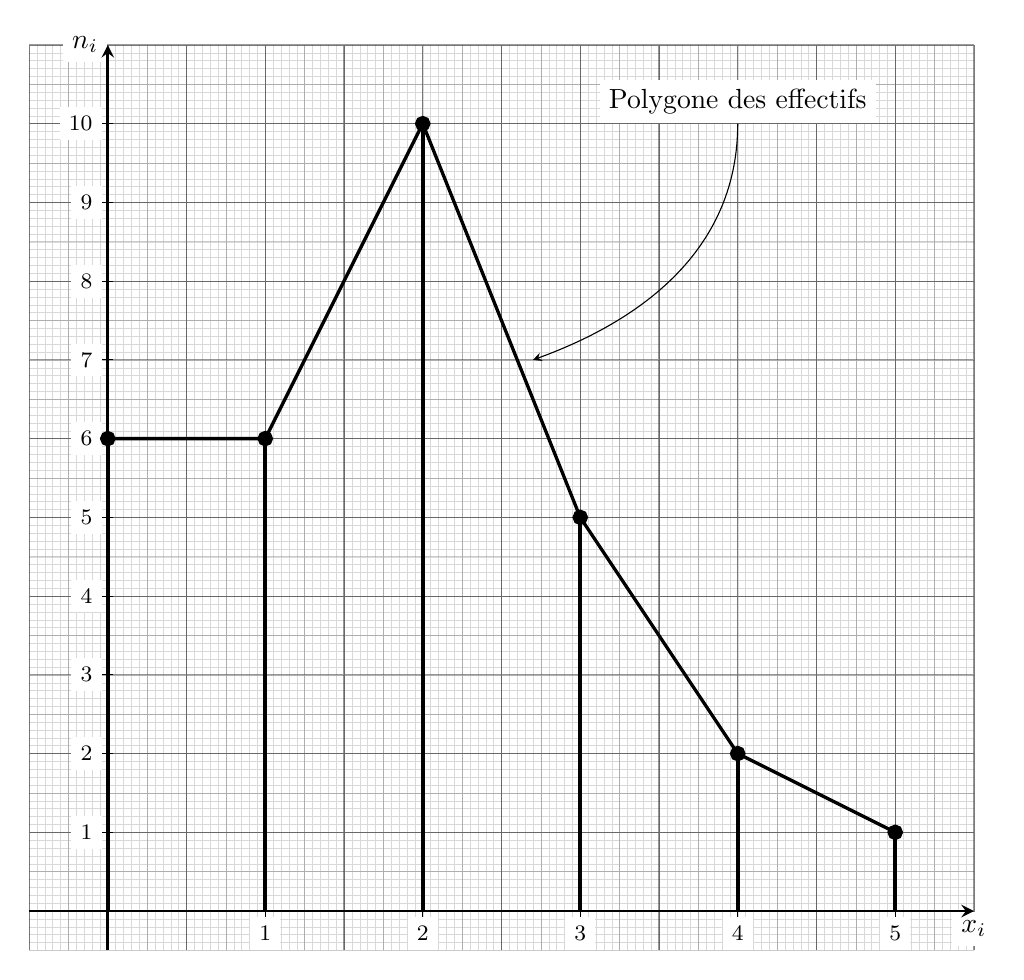
\begin{tikzpicture}[>=stealth,x=2.0cm,y=1.0cm,ybar,ycomb]
                                    \draw [color=black, xstep=1.0cm,ystep=1.0cm, line width=.4pt, opacity=.4] 
                                          (-0.5,-0.5) grid (5.5,11);
                                    \draw [color=black, xstep=0.5cm,ystep=0.5cm, line width=.2pt, opacity=.2] 
                                          (-0.5,-0.5) grid (5.5,11);
                                    \draw [color=black, xstep=0.1cm,ystep=0.1cm, line width=.15pt, opacity=.15] 
                                          (-0.5,-0.5) grid (5.5,11);
                                    \draw[] (0,11) node[fill=white, left] {$n_i$};
                                    \draw[] (5.5,0) node[fill=white, below] {$x_i$};
                                    \draw[->,color=black, line width=1pt] (-0.5,0) -- (5.5,0);
                                    \foreach \x in {1,2,...,5}
                                    \draw[shift={(\x,0)},color=black] (0pt,2pt) -- (0pt,-2pt) 
                                          node[below,fill=white] {\footnotesize $\x$};
                                    \draw[->,color=black, line width=1pt] (0,-0.5) -- (0,11);
                                    \foreach \y in {1,2,...,10}
                                    \draw[shift={(0,\y)},color=black] (2pt,0pt) -- (-2pt,0pt) 
                                          node[left,fill=white] {\footnotesize $\y$};
                                    \draw[ultra thick]
                                          plot[ycomb,thin,mark=*] coordinates{(0,6) (1,6) (2,10) (3,5) (4,2) (5,1)};
                                    \draw[very thick] (0,6) -- (1,6) -- (2,10) -- (3,5) -- (4,2) -- (5,1);
                                    \draw[] (4,10) node[fill=white, above] {Polygone des effectifs};
                                    \draw[->] (4,10) to[out=-90,in=20] (2.7,7);
                              \end{tikzpicture}
                              \caption{Diagramme en b\^atons repr\'esentant le tableau~\ref{tab:variable discret}.}
                              \label{fig:diagramme en batons}
                        \end{figure}
                  %
                  \subsubsection{Histogramme}
\index{Histogramme}
                        Consid\'erons le tableau~\ref{tab:variable continue}.
                        On a regroup\'e les donn\'ees par classe d'amplitude 5~cm. \newline
                        \begin{table}[h!]
                        \centering
                              \begin{tabular}{|c|c|c|}
                              \hline
                              Classes       & Effectifs    & Centre  \\
                              \hline
                              [150 ; 155[   &       2      &  152.5  \\
                              \hline
                              [155 ; 160[   &       4      &  157.5  \\
                              \hline
                              [160 ; 165[   &       5      &  162.5  \\
                              \hline
                              [165 ; 170[   &       8      &  167.5  \\
                              \hline
                              [170 ; 175[   &       4      &  172.5  \\
                              \hline
                              [175 ; 180[   &       3      &  177.5  \\
                              \hline
                              [180 ; 185[   &       2      &  182.5  \\
                              \hline
                              [185 ; 190[   &       1      &  187.5  \\
                              \hline
                              \end{tabular}
                        \caption{Tableau pr\'esentant les tailles en centim\`etres des \'el\`eves d'une classe de terminale.}
                        \label{tab:variable continue}
                        \end{table}
                        %
                        Cette s\'erie peut \^etre repr\'esent\'ee graphiquement par le diagramme~\ref{fig:histogramme}.
                        %
                        \begin{figure}%[h!]
                        \centering
                              \begin{tikzpicture}[>=stealth,x=1.0cm,y=1.0cm,ybar interval]
                                    \draw [color=black, xstep=1.0cm,ystep=1.0cm, line width=.4pt, opacity=.4] 
                                          (-0.5,-0.5) grid (10,9.5);
                                    \draw [color=black, xstep=0.5cm,ystep=0.5cm, line width=.2pt, opacity=.2] 
                                          (-0.5,-0.5) grid (10,9.5);
                                    \draw [color=black, xstep=0.1cm,ystep=0.1cm, line width=.15pt, opacity=.15] 
                                          (-0.5,-0.5) grid (10,9.5);
                                    \draw[] (0,9.5) node[fill=white, left] {$n_i$};
                                    \draw[] (10,0) node[fill=white, below] {$x_i$};
                                    \draw[->,color=black, line width=1pt] (-0.5,0) -- (10,0);
                                    \foreach \x/\xtext in {1/150,2/155,3/160,4/165,5/170,6/175,7/180,8/185,9/190}
                                    \draw[shift={(\x,0)},color=black] (0pt,2pt) -- (0pt,-2pt) 
                                          node[below,fill=white] {\footnotesize \rotatebox{90}{$\xtext$}};
                                    \draw[->,color=black, line width=1pt] (0,-0.5) -- (0,9.5);
                                    \foreach \y in {1,2,...,8}
                                    \draw[shift={(0,\y)},color=black] (2pt,0pt) -- (-2pt,0pt) 
                                          node[left,fill=white] {\footnotesize $\y$};
                                    \draw[color=loko2!50!black,fill=loko1!80,fill opacity=.5, ultra thick]
                                          plot coordinates{(1,2) (2,4) (3,5) (4,8) (5,4) (6,3) (7,2) (8,1) (9,1)};
                                    \draw[ultra thick]
                                          (1.5,2) -- (2.5,4) -- (3.5,5) -- (4.5,8) -- (5.5,4) 
                                                  -- (6.5,3) -- (7.5,2) -- (8.5,1);
                                    \foreach \x/\y in {1.5/2,2.5/4,3.5/5,4.5/8,5.5/4,6.5/3,7.5/2,8.5/1}
                                          \filldraw (\x,\y) circle (2pt);
                                    \draw[] (8,8) node[fill=white, above] {Polygone des effectifs};
                                    \draw[->] (8,8) to[out=-90,in=20] (5.5,5);
                              \end{tikzpicture}
                              \caption{Histogramme repr\'esentant la s\'erie statistique de 
                                       la table~\ref{tab:variable continue}}
                              \label{fig:histogramme}
                        \end{figure}
                        \nota{
                              Dans un histogramme, 
                              il est souvent pr\'ef\'erable de travailler avec des classes d'amplitudes constantes.
                              Dans le cas o\`u les amplitudes des classes sont diff\'erentes,
                              l'effectif doit \^etre proportionnel \`a l'aire (et non \`a la hauteur).
                        }
                  %
                  \subsubsection{Diagramme en secteur}
\index{Diagramme!en secteur}                  
                        Le tableau~\ref{tab:religions} indique les religions les plus pratiqu\'ees
                        ainsi que le nombre de pratiquants en 2010.
                        
                        \begin{table}[h!]
                        \centering
                              \begin{tabular}{|c|c|c|c|}
                              \hline 
                              Religions & Nombre de   & Pourcentages & Angle du secteur \\ 
                                        & pratiquants &              &  correspondant   \\
                              \hline 
                              Christianisme & 2\,420 & 36,24 & 130,5 \\ 
                              \hline 
                              Islam & 1\,800 & 26,95 & 97,04 \\ 
                              \hline 
                              Sans religion & 1\,150 & 17,22 & 61,99 \\ 
                              \hline 
                              Hindouisme & 520 & 7,79 & 28 \\ 
                              \hline 
                              Bouddhisme & 400 & 5,99 & 21,56 \\ 
                              \hline 
                              Autres & 388 & 5,81 & 20,92 \\ 
                              \hline 
                              \end{tabular} 
                              \caption{Tableau indiquant les religions les plus pratiqu\'es 
                                       ainsi que le nombre de pratiquants (en millions) en 2010.}
                              \label{tab:religions}
                        \end{table}
                        %
                        Ce tableau peut \^etre repr\'esent\'e par un diagramme en secteur 
                        comme dans la figure~\ref{fig:religions}.
                        \begin{figure}[H]
                        \centering
                              \begin{tikzpicture}[scale=4.5]
                                    \draw[very thick] (0,0) circle (1);
                                    \filldraw[fill=white] (0,0) -- (1,0) arc (0:130.5:1) -- cycle ; 
                                    \filldraw[fill=loko1] (0,0) -- (130.5:1) arc (130.5:227.49:1) -- cycle ; 
                                    \filldraw[fill=black] (0,0) -- (227.49:1) arc (227.49:289.49:1) -- cycle ; 
                                    \filldraw[fill=loko3] (0,0) -- (289.49:1) arc (289.49:317.52:1) -- cycle ; 
                                    \filldraw[fill=loko1!50!loko5] (0,0) -- (317.52:1) arc (317.52:339.08:1) -- cycle ; 
                                    \filldraw[fill=loko6] (0,0) -- (339.08:1) arc (339.08:360:1) -- cycle ; 
                                    \draw[black] ( 65:.55) node{Christianisme};
                                    \draw[white] (190:.60) node{Islam};
                                    \draw[white] (255:.65) node{Irreligion};
                                    \draw[white] (306:.82) node{Hindouisme};
                                    \draw[black] (332:.78) node{Bouddhisme};
                                    \draw[black] (350:.80) node{Autres};
                              \end{tikzpicture}
                              \caption{Diagramme en secteurs indiquant les religions les plus pratiqu\'es.}
                              \label{fig:religions}
                        \end{figure}
                  %
                  \subsection{Caract\'eristiques de positions}
                        \begin{defi}
                              \begin{itemize}
                                    \item Dans le cas d'une variable discr\`ete,
\index{mode}
                                          le \emph{mode} correspond \`a la valeur du caract\`ere 
                                          ayant l'effectif le plus \'elev\'e.
                                    \item Dans le cas d'une variable continue,
\index{classe modale}
                                          la \emph{classe modale} d\'esigne la classe 
                                          qui correspond \`a l'effectif le plus \'elev\'e.
                                    \item La \emph{m\'ediane} est la valeur du caract\`ere qui partage
\index{mediane@m\'ediane}
                                          la s\'erie en deux groupes de m\^eme effectif.
                                          \begin{ex}
                                                \begin{itemize}
                                                      \item On consid\`ere l'\^age de dix personnes
                                                            rang\'ees par ordre croissant :
                                                            \begin{center}
                                                                  15 \hspace{\stretch{1}}
                                                                  16 \hspace{\stretch{1}}
                                                                  16 \hspace{\stretch{1}}
                                                                  17 \hspace{\stretch{1}}
                                                                  17 \hspace{\stretch{1}}
                                                                  18 \hspace{\stretch{1}}
                                                                  18 \hspace{\stretch{1}}
                                                                  18 \hspace{\stretch{1}}
                                                                  19 \hspace{\stretch{1}}
                                                                  19 .
                                                                  ~\\[\baselineskip]
                                                            \end{center}
                                                            On peut prendre comme m\'ediane le milieu de $]17 ; 18[$
                                                            soit $17,5$ ; c'est-\`a-dire 17 ans et 6 mois.
                                                            Ce n'est pas n\'ecessaire ; 
                                                            toute valeurs entre 17 et 18 divise la s\'erie en deux.
                                                      \item Consid\'erons le tableau~\ref{tab:veufs}, 
                                                            montrant le nombre de veufs
                                                            dans une ville class\'e par cat\'egorie d'\^age.
                                                            \begin{table}[H]
                                                            \centering
                                                            \begin{tabular}{|c|c|c|}
                                                            \hline 
                                                            Classes ($c_i$) & Effectifs ($n_i$) & 
                                                                  Effectifs cumul\'e croissant ($n_i\uparrow$) \\
                                                            \hline 
                                                            - de 30 & 15 & 15 \\ 
                                                            \hline 
                                                            [30 ; 40[ & 48 & 63 \\ 
                                                            \hline             
                                                            [40 ; 50[ & 169 & 232 \\ 
                                                            \hline 
                                                            [50 ; 60[ & 432 & 664 \\ 
                                                            \hline 
                                                            [60 ; 70[ & 858 & 1522 \\ 
                                                            \hline 
                                                            [70 ; 80[ & 1388 & 2910 \\ 
                                                            \hline 
                                                            [80 ; 90[ & 808 & 3718 \\ 
                                                            \hline 
                                                            90 et + & 118 & 3836 \\ 
                                                            \hline 
                                                            \end{tabular} 
                                                            \caption{Tableau repr\'esentant le nombre de veufs dans une ville.}
                                                            \label{tab:veufs}
                                                            \end{table}
                                                            
                                                            Le total des effectifs est 3~836 et la m\'ediane qui correspond
                                                            \`a un effectif $\frac{N}{2} = 1918$ est atteinte dans la classe 
                                                            [70 ; 80[.
                                                            Comme l'effectif cumul\'e correspondant \`a la classe moins de 70
                                                            est de 1522 et celui de la classe moins de 80 est de 2910,
                                                            on interpole lin\'eairement dans la classe [70 ; 80[.
                                                            La m\'ediane est alors
                                                            \footnote{%
                                                              \TCDSideBySide[.27]{%
                                                                \centering
                                                                \begin{tikzpicture}[scale=.2]
                                                                  \draw[loko1,dashed] (-5,0) -- (5,0);
                                                                  \draw[loko2] (-5,-2.5) -- (5,2.5);
                                                                  \draw[loko2] (-3,-1.5) circle (1pt);
                                                                  \draw[loko2] (3,1.5) circle (1pt);
                                                                  \draw[loko2] (0,0) circle (1pt);
                                                                  \draw[black] (-3,-1.5) -- (-3,-2.5) node[below] {$a$};
                                                                  \draw[black] (3,1.5) -- (3,-2.5) node[below] {$b$};
                                                                  \draw[dashed] (-3,-1.5) -- (5,-1.5) node[right] {$\alpha$};
                                                                  \draw[dashed] (3,1.5) -- (5,1.5) node[right] {$\beta$};
                                                                  \draw[loko1] (-5,0) node[fill=white] {$m$};
                                                                  \draw[loko1] (0,0) -- (0,-2.5) node[below] {$x_m$};
                                                                \end{tikzpicture}%
                                                              }{%
                                                                Équation de la droite oblique :
                                                                \[
                                                                  y=\frac{\beta-\alpha}{b-a}(x-a)+\alpha.
                                                                \]
                                                                On en déduit
                                                                \[
                                                                  x=\frac{b-a}{\beta-\alpha}(y-\alpha)+a.
                                                                \]
                                                                Pour trouver $x_m$, on prend $y=m$ :
                                                                \[
                                                                  \propbox{x_m=\frac{b-a}{\beta-\alpha}(m-\alpha)+a}.
                                                                \]
                                                              }%
                                                            } :
                                                            \[
                                                                  70 + \frac{80 - 70}{1388} \cdot (1918 - 1522)
                                                                   = 72,853\text{ ans}            
                                                            \]
                                                            soit 72 ans 10 mois et 7 jours.%
                                                \end{itemize}
                                          %
                                          \end{ex}
                                    \item La \emph{moyenne arithm\'etique simple} est 
\index{Moyenne!arithmetique@arithm\'etique!simple}
                                          \[
                                          \bar{x} = \frac{x_1 + x_2 + \cdots + x_n}{N}.
                                          \]
                                    \item La \emph{moyenne arithm\'etique pond\'er\'ee} est 
\index{Moyenne!arithmetique@arithm\'etique!ponderee@pond\'er\'ee}
                                          \[
                                          \bar{x} = \frac{k_1 \cdot x_1 + k_2 \cdot x_2 + \cdots + k_n \cdot x_n}{N}.
                                          \]
                                          \begin{ex}
                                                \begin{itemize}
                                                      \item Les notes de math\'ematiques d'un \'el\`eve durant le premier 
                                                            trimestre sont : 8, 12 et 13.
                                                            La moyenne (simple) est donc $\frac{8 + 12 + 13}{3} = 11$.
                                                      \item Les notes d'un \'el\`eve au premier trimestre sont repr\'esent\'es
                                                            dans le tableau~\ref{tab:notes}.
                                                            \begin{table}[H]
                                                                  \centering
                                                                  \begin{tabular}{|c|c|c|}
                                                                  \hline
                                                                        Mati\`eres        & Notes/20 & Coefficients \\
                                                                  \hline
                                                                        Malagasy          &    14    &     3        \\
                                                                        Fran\c{c}ais      &    13    &     2        \\
                                                                        Anglais           &    14    &     1        \\
                                                                        Philosophie       &    12    &     2        \\
                                                                        Histo-g\'eo       &    11    &     2        \\
                                                                        Math\'ematiques   &    16    &     4        \\
                                                                        Physique          &    13    &     4        \\
                                                                        SVT               &    15    &     4        \\
                                                                        EPS               &    08    &     1        \\
                                                                  \hline
                                                                  \end{tabular}
                                                                  \caption{Notes d'un \'el\`eve en s\'erie scientifique.}
                                                                  \label{tab:notes}
                                                            \end{table}
                                                            
                                                            La moyenne est donc : 
                                                            $\displaystyle{
                                                                  \frac{  3 \cdot 14 + 2 \cdot 13 + 1 \cdot 14
                                                                        + \cdots
                                                                        + 4 \cdot 15 + 1 \cdot 08 }
                                                                       {3 + 2 + 1 + \cdots + 4 + 1}
                                                            }$
%                                                            $
%                                                                  \frac{  3 \cdot 14 + 2 \cdot 13 + 1 \cdot 14
%                                                                        + 2 \cdot 12 + 2 \cdot 11 + 4 \cdot 16
%                                                                        + 4 \cdot 13 + 4 \cdot 15 + 1 \cdot 08 }
%                                                                       {3 + 2 + 1 + 2 + 2 + 4 + 4 + 4 + 1}
%                                                            $
                                                            qui est \'egale \`a $13,57$.
                                                \end{itemize}
                                          \end{ex}
                                    \item Les \emph{quartiles} $Q1$, $Q2$ et $Q3$ sont les trois valeurs 
\index{Quartiles}
                                          du caract\`ere qui partagent la s\'erie en quatre groupes de m\^eme effectif.
                                          \begin{ex}
                                                On donne le tableau~\ref{tab:quartiles}.
                                                \begin{table}[H]
                                                \[
                                                      \begin{array}{|c|c|c|c|}
                                                      \hline
                                                      x_i      & n_i      & n_i \uparrow & n_i \downarrow \\
                                                      \hline
                                                      7        & 4        & 4            & 27             \\
                                                      8        & 1        & 5            & 23             \\
                                                      9        & 2        & 7            & 22             \\
                                                      10       & 3        & 10           & 20             \\
                                                      11       & 3        & 13           & 17             \\
                                                      12       & 1        & 14           & 14             \\
                                                      13       & 5        & 19           & 13             \\
                                                      14       & 3        & 22           &  8             \\
                                                      15       & 4        & 26           &  5             \\
                                                      16       & 1        & 27           &  1             \\
                                                      \hline
                                                      \end{array}
                                                \]
                                                \caption{Tableau repr\'esentant des donn\'ees inconnues.}
                                                \label{tab:quartiles}
                                                \end{table}
                                                On a $N = 27$ et donc $\frac{N}{4} = 6,75$.
                                                Comme $Q1$ doit \^etre une valeur de la s\'erie, on prend la valeur de rang $7$
                                                (premier entier sup\'erieur ou \'egal \`a $6,75$) ; de m\^eme
                                                $\frac{N}{2} = 13,5$ donne le rang $14$ et $\frac{3N}{4} = 20,25$ le rang $21$.
                                                En lisant les effectifs cumul\'es croissants, on a alors :
                                                \begin{itemize}
                                                      \item $Q1 = 9$,
                                                      \item $Q2 = 12$ (c'est la m\'ediane),
                                                      \item $Q3 = 14$.
                                                \end{itemize}
                                          \end{ex}
                                          ~\\%[\baselineskip]
                                               \smallnota{Avec la convention adopt\'ee ici, et contrairement \`a la m\'ediane, les quartiles doivent
                                                     n\'ec\'essairement \^etre des valeurs de la s\'erie.
                                                     Dans le cas o\`u $N/4$ n'est pas un nombre entier,
                                                     on prend le plus petit entier sup\'erieur (par exemple 7 pour 6,75).}
                                    \item L'\emph{interquartile} est $Q3 - Q1$.
\index{Interquartiles}
                                    \item Les \emph{d\'eciles} $D1$, $D2$, \ldots , $D9$ sont les valeurs
                                          partageant la s\'erie en dix groupes de m\^eme effectif.
\index{Deciles@D\'eciles}
                              \end{itemize}
                        \end{defi}
                  %
                  \subsection{Caract\'eristique de dispersion}
                        La variance est la moyenne des carr\'es des \'ecarts \`a la moyenne, elle est d\'efinie par : 
\index{Variance}
                        \begin{center}
                              \defbox{
                                    \[
                                          \sigma^2 = \frac{1}{N} \cdot \sum n_i \cdot (x_i - \bar{x})^2 .
                                    \]
                              }
                        \end{center}
                        L'\'ecart-type est la racine carr\'ee de la variance.
\index{Ecart-type@\'Ecart-type}                        
                        \begin{ex}
                              On consid\`ere le tableau~\ref{tab:variance}.
                              \begin{table}[H]
                                    \centering
                                    \begin{tabular}{|c|c|c|c|c|c|}
                                    \hline 
                                    $x_i$ & $n_i$ & $c_i$ & $c_i - \bar{x}$ & $(c_i - \bar{x})^2$ & $n_i \cdot (c_i - \bar{x})^2$ \\ 
                                    \hline 
                                    [0;4[ & 4 & 2 & -8,76 & 73,7376 & 306,9504 \\ 
                                    \hline 
                                    [4;8[ & 20 & 6 & -4,76 & 22,6576 & 453,152 \\ 
                                    \hline 
                                    [8;12[ & 40 & 10 & -0,76 & 0,5776 & 23,104 \\ 
                                    \hline 
                                    [12;16[ & 25 & 14 & 3,24 & 10,4976 & 262,44 \\ 
                                    \hline 
                                    [16;20[ & 11 & 18 & 7,24 & 52,4176 & 576,5936 \\ 
                                    \hline 
                                    Total : & 100 &   &   &   & 1622,24 \\ 
                                    \hline 
                                    \end{tabular} 
                                    \caption{Notes des \'el\`eves dans une classe de terminale.}
                                    \label{tab:variance}
                              \end{table}
                              On a $\bar{x} = \frac{1}{N} \cdot \sum n_i \cdot c_i$ et 
                              $\sigma^2 = \frac{1622,24}{100} = 16,2224$.
                              Ainsi, $\sigma = \sqrt{16,2224} = 4,0277$.
                        \end{ex}
                        Plus l'\'ecart-type est faible, plus la moyenne est repr\'esentative de la s\'erie.
%
      \section{S\'eries statistiques \`a deux variables}
      		\subsection{D\'efinitions}
            \begin{defi}
                  Soient $x$ et $y$ deux caract\`eres quantitatifs d'une m\^eme population.
                  A chaque individu de la population, on associe un couple $(x_i ; y_i)$ 
                  o\`u $x_i$ et $y_i$ sont les valeurs prises par les variables $x$ et $y$ respectivement.
                  
                  Dans un rep\`ere $(O ; \vec{\imath} , \vec{\jmath})$, l'ensemble des points $M_i (x_i ; y_i)$
                  est appel\'e \emph{nuage de points} associ\'e \`a la s\'erie statistique.
                  
                  Soit une s\'erie statistique \`a deux variables $x$ et $y$ de moyenne $\bar{x}$ et $\bar{y}$.
                  Le point $G$ de coordonn\'ees $(\bar{x} ; \bar{y})$ est appel\'e \emph{point moyen}
                  du nuage de points associ\'e \`a la s\'erie statistique.
                  
                  On appelle \emph{covariance} de $x$ et $y$ le nombre $\sigma_{xy}$ d\'efini par
                  \par\smallskip\noindent
                  \defbox{$\displaystyle
                        \begin{aligned}
                        \sigma_{xy}
                           &=\frac{1}{n}\sum_{i=1}^{n}(x_i-\bar{x})(y_i-\bar{y}) \\
                           &=\frac{1}{n}\sum_{i=1}^{n}x_i y_i-\bar{x}\,\bar{y}.
                        \end{aligned}$}
                  \par\smallskip
                  \begin{ex}
                        Soit la s\'erie statistique double suivante :
	                        $x_i$ repr\'esente les salaires en milliers d'ariary propos\'es par diverses entreprises pour un poste,
	                        $y_i$ indique le nombre de candidats qui se sont pr\'esent\'es pour ces emplois.
                        \begin{tabular}{cccccc}
                              $x_i$ & 44 & 45 & 46 & 47 & 48 \\
                              $y_i$ & 10 & 13 & 17 & 19 & 21 
                        \end{tabular}.
                        On a $\bar{x} = \frac{44 + 45 + 46 + 47 + 48}{5} = 46$
                        et $\bar{y} = \frac{10 +  13 + 17 + 19 + 21}{5} = 16$ ; 
	                        ainsi, le point moyen est $G (46 ; 16)$.
                        
                        \begin{IEEEeqnarray*}{rCl}
                        \sigma_{xy} & = & \frac{1}{5}
                                      [
                                            (44-46)(10 - 16) + (45-46)(13-16) + (46-46)(17-16) \\
                                    &   & + (47-46)(19-16) + (48-46)(21-16) ] \\
                                    & = & 5,6.
                        \end{IEEEeqnarray*}
                        %
                        \begin{figure}[H]
                        \centering
                              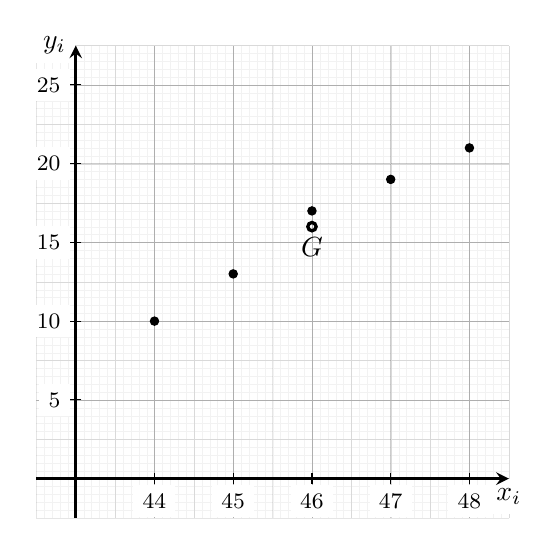
\begin{tikzpicture}[>=stealth,x=1.0cm,y=1.0cm,ybar,ycomb]
                                    \draw [xstep=0.1cm,ystep=0.1cm,opacity=.05,line width=.05]
                                          (-0.5,-0.5) grid (5.5,5.5);
                                    \draw [xstep=0.5cm,ystep=0.5cm,opacity=0.1,line width=0.1]
                                          (-0.5,-0.5) grid (5.5,5.5);
                                    \draw [xstep=1.0cm,ystep=1.0cm,opacity=0.2,line width=0.2]
                                          (-0.5,-0.5) grid (5.5,5.5);
                                    \draw[] (0,5.5) node[fill=white, left] {$y_i$};
                                    \draw[] (5.5,0) node[fill=white, below] {$x_i$};
                                    \draw[->,color=black, line width=1pt] (-0.5,0) -- (5.5,0);
                                    \foreach \x/\xtext in {1/44,2/45,3/46,4/47,5/48}
                                    \draw[shift={(\x,0)},color=black] (0pt,2pt) -- (0pt,-2pt) 
                                          node[below,fill=white] {\footnotesize $\xtext$};
                                    \draw[->,color=black, line width=1pt] (0,-0.5) -- (0,5.5);
                                    \foreach \y/\ytext in {1/5,2/10,3/15,4/20,5/25}
                                    \draw[shift={(0,\y)},color=black] (2pt,0pt) -- (-2pt,0pt) 
                                          node[left,fill=white] {\footnotesize $\ytext$};
                                    \foreach \x/\y in {1/2,2/2.6,3/3.4,4/3.8,5/4.2}
                                          \filldraw (\x,\y) circle (1.5pt);
                                    \draw[color = black, very thick] (3,3.2) circle (1.5pt) node[below] {$G$};
                              \end{tikzpicture}
                           \caption{Nuage de points et le point moyen $G$.}
                        \end{figure}
                  \end{ex}
            \end{defi}
            %
            \subsection{Ajustement affine}% (m\'ethode des moindres carr\'es)}
\index{Ajustement affine}
	                  Certaines s\'eries statistiques repr\'esentent des variables qui sont li\'ees.
                  Il est parfois possible de trouver une droite permettant d'approximer le nuage de points.
                  %
                  \subsubsection{Droite de r\'egression de $y$ en $x$}
\index{Droite de regression@Droite de r\'egression!de y en x@de $y$ en $x$}
	                        La droite de r\'egression obtenue par la m\'ethode des moindres carr\'es passe par le point moyen ;
                        ainsi, elle a une \'equation de la forme $y - \bar{y} = m (x - \bar{x})$ et le coefficient
                        directeur $m$ est \'egal \`a $\frac{\sigma_{xy}}{V(x)}$.
                  %
                  \subsubsection{Droite de r\'egression de $x$ en $y$}
\index{Droite de regression@Droite de r\'egression!de x en y@de $x$ en $y$}
                        Elle est donn\'ee par l'\'equation $x - \bar{x} = m' (y - \bar{y})$ et le coefficient
                        directeur $m'$ est \'egal \`a $\frac{\sigma_{xy}}{V(y)}$.
                  %
                  \subsubsection{Corr\'elation lin\'eaire}
\index{Correlation lineaire@Corr\'elation lin\'eaire}
                        Le coefficient de corr\'elation lin\'eaire sert \`a mesurer la relation entre les deux variables
                        $x$ et $y$.
                        Ce coefficient est donn\'e par \defbox{$\displaystyle{r = \frac{\sigma_{xy}}{\sigma_x \cdot \sigma_y}}$}.
                        \nota{
	                        Un coefficient de corr\'elation proche de $1$ ou $-1$ signifie que 
                        les deux variables sont << fortement corr\'el\'ees >>. \newline
	                        Comme $\sigma_x$, $\sigma_y$, $V(x)$ et $V(y)$ sont strictement positifs (aucune des deux variables n'est constante), 
                        les signes de $m$, $m'$ et $r$ d\'ependent de celui de $\sigma_{xy}$.
                              \begin{align*}
                                    m\cdot m' & = \frac{\sigma_{xy}}{V(x)} \cdot \frac{\sigma_{xy}}{V(y)}        
                                                = \frac{(\sigma_{xy})^2}{\sigma_x^2 \cdot \sigma_y^2}            
                                                = \left( \frac{\sigma_{xy}}{\sigma_x \cdot \sigma_y} \right)^2   
                                                = r^2.
                              \end{align*}
                        }
                  %
                  \subsubsection{Variances et calcul pratique}
\index{Variance}
                        Dans les formules ci-dessus, $V(x)$ et $V(y)$ d\'esignent les variances de $x$ et de $y$ :
                        \[
                        V(x) = \sigma_x^2 = \frac{1}{n}\sum_{i=1}^{n}(x_i - \bar{x})^2 = \frac{1}{n}\sum_{i=1}^{n} x_i^2 - \bar{x}^2 ,
                        \qquad
                        V(y) = \sigma_y^2 = \frac{1}{n}\sum_{i=1}^{n} y_i^2 - \bar{y}^2 .
                        \]
                        En pratique, on calcule $\sum x_i$, $\sum y_i$, $\sum x_i^2$, $\sum y_i^2$ et $\sum x_i y_i$ 
                        (dans un tableau ou \`a la calculatrice), puis les moyennes, les variances, la covariance,
                        les coefficients directeurs et $r$. On admet que le coefficient $r$ est toujours compris entre $-1$ et $1$.
                        \begin{ex}
                              Pour la s\'erie des salaires et des candidats ci-dessus : $\sum x_i^2 = 10\,590$ et 
                              $\sum y_i^2 = 1\,360$, donc $V(x) = \frac{10\,590}{5} - 46^2 = 2$ et $V(y) = \frac{1\,360}{5} - 16^2 = 16$.
                              La droite de r\'egression de $y$ en $x$ a pour coefficient directeur $m = \frac{5,6}{2} = 2,8$ ; 
                              son \'equation est $y - 16 = 2,8\,(x - 46)$, soit $y = 2,8\,x - 112,8$.
                              Enfin $r = \frac{5,6}{\sqrt{2}\times 4} \approx 0,99$ : la corr\'elation est forte et positive.
                        \end{ex}
                  %
                  \subsubsection{Ajustement apr\`es un changement de variable}
\index{Ajustement!exponentiel}
\index{Ajustement!logarithmique}
                        Lorsque le nuage de points a une forme nettement courbe, un ajustement affine de $y$ en $x$ 
                        n'est pas adapt\'e. On cherche alors une nouvelle variable pour laquelle le nuage est presque rectiligne,
                        on fait un ajustement affine sur cette nouvelle s\'erie, puis on revient aux variables de d\'epart.
                        \begin{itemize}
                              \item \emph{Ajustement exponentiel.} Si $y$ semble \^etre multipli\'e par un m\^eme nombre 
                                    quand $x$ augmente d'une m\^eme quantit\'e (croissance ou d\'ecroissance << en pourcentage >>),
                                    on pose $z = \ln y$ (les $y_i$ \'etant strictement positifs). Si la droite de r\'egression 
                                    de $z$ en $x$ est $z = a x + b$, alors $y = e^{ax + b} = B\, e^{ax}$ avec $B = e^{b}$.
                              \item \emph{Ajustement logarithmique.} Si $y$ augmente d'une m\^eme quantit\'e chaque fois que 
                                    $x$ est multipli\'e par un m\^eme nombre, on pose $t = \ln x$ (les $x_i$ \'etant strictement positifs).
                                    Si la droite de r\'egression de $y$ en $t$ est $y = a t + b$, alors $y = a \ln x + b$.
                              \item D'autres changements de variable sont possibles, par exemple $X = x^2$ ou $Y = \frac{1}{y}$ ;
                                    l'\'enonc\'e indique en g\'en\'eral celui qu'il faut utiliser.
                        \end{itemize}
                        On compare les coefficients de corr\'elation des deux s\'eries pour juger quel ajustement est le meilleur.
                  %
                  \subsubsection{Pr\'evisions}
\index{Prevision@Pr\'evision}
                        Une fois l'ajustement choisi, son \'equation permet d'estimer une valeur de $y$ pour une valeur de $x$ donn\'ee
                        (et inversement). On parle d'\emph{interpolation} si $x$ est dans l'intervalle des valeurs observ\'ees
                        et d'\emph{extrapolation} sinon ; une extrapolation suppose que la tendance observ\'ee se poursuit,
                        ce qui n'est jamais certain.
                        \nota{
                        Une pr\'evision n'a de sens que si l'ajustement est de bonne qualit\'e, c'est-\`a-dire si $|r|$ est
                        proche de $1$ (un usage courant est d'exiger $|r| \geq 0,87$, soit environ $\frac{\sqrt{3}}{2}$). \newline
                        Pour estimer $y$ connaissant $x$, on utilise la droite de r\'egression de $y$ en $x$ ;
                        pour estimer $x$ connaissant $y$, on utilise de pr\'ef\'erence celle de $x$ en $y$.
                        Les deux droites passent par le point moyen $G$ et sont d'autant plus proches que $|r|$ est proche de $1$.
                        }

\TCDLessonStyleOff
\clearpage
\providecommand{\cov}[2]{\mathrm{Cov}\left( #1 , #2 \right)}
\providecommand{\var}[1]{\mathrm{Var}\left( #1 \right)}
\section{Exercices}
      \begin{exo}
            \label{exo:stat1}
            Pour chacune des variables statistiques suivantes, dire si elle est qualitative ou quantitative ; 
            dans le cas d'une variable quantitative, dire si elle est discr\`ete ou continue.
            \begin{enumerate}
                  \item Couleur des yeux des \'el\`eves,
                  \item nombre d'enfants dans chaque foyer,
                  \item poids de nouveaux-n\'es dans un h\^opital,
                  \item nationalit\'es des participants \`a un championnat,
                  \item tailles des \'etudiants d'un lyc\'ee.
            \end{enumerate}
      \end{exo}
      %
      \begin{exo}
            \label{exo:stat2}
            Le tableau suivant donne la répartition selon le groupe sanguin de 60 individus pris au hasard.
            \begin{table}[H]
                  \centering
                        \begin{tabular}[b]{|c|c|c|c|c|}
                        \hline 
                        Groupes & O & A & B & AB \\ 
                        \hline 
                        Effectif & 10 & 22 & 17 & $n_{AB}$ \\ 
                        \hline 
                  \end{tabular}. 
            \end{table}
            \begin{enumerate}
                  \item Déterminer la variable statistique et son type.
                  \item Déterminer l’effectif des personnes ayant un groupe sanguin AB.
                  \item Repr\'esenter cette variable dans un diagramme en b\^aton
                        puis dans un diagramme en secteur.
            \end{enumerate}
      \end{exo}
      %
      \begin{exo}
            \label{exo:stat3}
	            On a relevé, pour un article particulier, le nombre d’articles vendus par jour dans un magasin.
	            Voici les nombres obtenus :
	            \begin{center}
	            \adjustbox{max width=\linewidth}{\begin{tabular}{lllllllllllllll}
                  $19$ & $24$ & $23$ & $20$ & $18$ & $19$ & $22$ & $25$ & $24$ & $23$ & $17$ & $21$ & $23$ & $19$ & $22$  \\
                  $19$ & $19$ & $21$ & $23$ & $20$ & $17$ & $21$ & $18$ & $21$ & $18$ & $22$ & $21$ & $20$ & $23$ & $20$  \\
                  $18$ & $19$ & $23$ & $22$ & $18$ & $19$ & $20$ & $20$ & $19$ & $20$ & $17$ & $19$ & $25$ & $26$ & $20$  \\
                  $23$ & $18$ & $20$ & $21$ & $21$ & $21$ & $22$ & $23$ & $22$ & $17$ & $16$ & $20$ & $22$ & $25$ & $20$  \\
	            \end{tabular}}
	            \end{center}
            %
            \begin{enumerate}
	                  \item Quelle est la variable \'etudi\'ee\,?
                  \item Dresser le tableau statistique repr\'esentant cette variable,
	                        en y indiquant les effectifs, la fr\'equence, la fr\'equence cumul\'ee ainsi que les effectifs cumul\'es.
                  \item Tracer le diagramme en b\^aton associ\'e \`a cette variable.
                  \item D\'eterminer le mode ainsi que la m\'ediane.
                  \item Calculer la moyenne arithm\'etique, la variance ainsi que l'\'ecart-type.
            \end{enumerate}
      \end{exo}
      %
      \begin{exo}
            \label{exo:stat4}
            Les moyennes g\'en\'erales des \'etudiants d'un lyc\'ee sont les suivantes : \newline
            \begin{tabular}[b]{rrrrrrrrrrrrrrr}
                  $9.46$ & $9.13$ & $13.61$ & $11.61$ & $9.06$ & $8.38$ & $10.64$ & $8.66$ & $14.56$ \\
                  $11.51$ & $10.96$ & $12.54$ & $10.00$ & $14.34$ & $13.17$ & $8.13$ & $9.01$ & $8.33$ \\
                  $6.82$ & $11.40$ & $9.43$ & $12.12$ & $10.16$ & $12.67$ & $6.55$ & $7.58$ & $5.72$ \\
                  $11.34$ & $12.88$ & $8.12$ & $8.79$ & $15.27$ & $8.26$ & $9.83$ & $8.33$ & $9.32$ \\
            \end{tabular}.
            %
            \begin{enumerate}
	                  \item Quelle est la variable \'etudi\'ee\,?
                  \item Dresser le tableau statistique repr\'esentant cette variable,
                        mettez-y les classes, les effectifs, la fr\'equence, la fr\'equence cumul\'ee ainsi que les effectifs cumul\'es.
                        (On prendra des classes d'amplitude 2 en commen\c{c}ant par $[5,5 \ ; \ 7,5[$.)
                  \item Tracer un histogramme associ\'e \`a cette variable.
                  \item D\'eterminer le mode ainsi que la m\'ediane.
                  \item Calculer la moyenne arithm\'etique, la variance ainsi que l'\'ecart-type.
            \end{enumerate}
      \end{exo}
      %
      \begin{exo}
            \label{exo:stat5}
            Un boulanger vend des pains qui doivent peser 200~g.
            Cependant, la perfection n'est pas de ce monde et les poids de son pain varient.
            Voici les poids (en grammes) de 56 pains pris au hasard :
            \begin{center}
            \adjustbox{max width=\linewidth}{%
            \begin{tabular}{llllllll}
                  $200.9$ & $198.8$ & $200.4$ & $199.5$ & $201.3$ & $200.8$ & $199.1$ & $202.8$ \\
                  $199.7$ & $200.9$ & $202.5$ & $200.9$ & $200.0$ & $200.3$ & $200.0$ & $198.8$ \\
                  $199.5$ & $199.6$ & $200.3$ & $198.3$ & $200.0$ & $201.4$ & $200.6$ & $200.0$ \\
                  $199.2$ & $199.7$ & $201.2$ & $200.2$ & $200.1$ & $199.2$ & $201.2$ & $200.5$ \\
                  $200.7$ & $198.8$ & $199.7$ & $198.4$ & $196.7$ & $198.6$ & $197.4$ & $201.1$ \\
                  $199.1$ & $201.5$ & $197.1$ & $200.3$ & $200.6$ & $200.7$ & $200.2$ & $199.9$ \\
                  $198.0$ & $202.9$ & $199.3$ & $199.2$ & $199.9$ & $201.7$ & $201.5$ & $198.4$ \\
            \end{tabular}%
            }
            \end{center}
            %
            \begin{enumerate}
	                  \item Quelle est la variable \'etudi\'ee\,?
                  \item Dresser le tableau statistique repr\'esentant cette variable,
                        mettez-y les classes, les effectifs, la fr\'equence, la fr\'equence cumul\'ee ainsi que les effectifs cumul\'es.
                        (On prendra des classes d'amplitude 1~g en commen\c{c}ant par $[196 ; 197[$.)
                  \item Tracer un histogramme associ\'e \`a cette variable.
                  \item D\'eterminer le mode ainsi que la m\'ediane.
                  \item Calculer la moyenne arithm\'etique, la variance ainsi que l'\'ecart-type.
            \end{enumerate}
      \end{exo}
      %
      \begin{exo}
            \label{exo:stat6}
            Une usine produit des pièces d'une machine. 
            Pour chaque pièce (individu), on dispose du coût de sa production (en milliers d'ariary) et 
            du temps nécessaire pour sa réalisation (en heures). 
            Le tableau ci-après (série statistique) donne cette répartition : \newline
            \begin{tabular}[b]{|c|c|c|c|c|c|}
                        \hline 
                  Individu & 1 & 2 & 3 & 4 & 5 \\ 
                        \hline 
                  Temps ($X$) mesur\'e en heures & 2 & 3 & 5 & 2 & 4 \\ 
                        \hline 
                  Co\^ut ($Y$) mesur\'e en milliers d'Ariary & 10 & 16 & 23 & 12 & 18 \\ 
                        \hline 
            \end{tabular}. \newline
            On rappelle les formules suivantes :
            \begin{itemize}
                  \item $\cov{X}{Y} 
                        = \displaystyle{\frac{1}{N} \sum_{i=1}^{N} \left[ (x_i - \bar{x}) (y_i - \bar{y} ) \right]}$,
                  \item $r = \frac{\cov{X}{Y}}{\sigma(X) \sigma(Y)}$,
                  \item Droite de r\'egression de $Y$ en $X$ :
                        $Y = \frac{\cov{X}{Y}}{\var{X}} \cdot \left( X - \bar{x} \right) + \bar{y}$.
            \end{itemize}
            
            \begin{enumerate}
                  \item Calculer la moyenne de la variable statistique $X$.
                  \item Calculer la moyenne de la variable statistique $Y$.
                  \item Calculer l'\'ecart-type de la variable statistique $X$.
                  \item Calculer l'\'ecart-type de la variable statistique $Y$.
                  \item Calculer la covariance des variables statistiques $X$ et $Y$.
                  \item En supposant qu'il existe une corr\'elation entre $X$ et $Y$, 
                        d\'eterminer la droite de r\'egression de $Y$ en $X$.
                  \item Calculer le coefficient de corr\'elation. Conclusion\,?
                  \item Une nouvelle pièce est réalisée en 6 heures. 
                        Estimer le coût de production de cette pièce en utilisant la droite de régression établie.
            \end{enumerate}
      \end{exo}
%%%%%%%%%%%%%%%%%%%%%%%%%%%%%%%%%%%%%%%%%%%%%%%%%%%%%%%%%%%%%%%%%%%%%%%%%
%%%%%%%%%%%%%%%%%%%%%%%%%%%%%%%%%%%%%%%%%%%%%%%%%%%%%%%%%%%%%%%%%%%%%%%%%
      %
      \begin{exo}
            \label{exo:stat7}
            Une coop\'erative rizicole compare, sur six parcelles comparables, la quantit\'e d'engrais $x$ 
            (en kilogrammes par hectare) et le rendement $y$ (en quintaux par hectare) obtenu \`a la r\'ecolte.
            \begin{center}
            \begin{tabular}{|c|c|c|c|c|c|c|}
                  \hline
                  Engrais $x_i$ (kg/ha) & 0 & 20 & 40 & 60 & 80 & 100 \\
                  \hline
                  Rendement $y_i$ (q/ha) & 22 & 27 & 30 & 35 & 37 & 41 \\
                  \hline
            \end{tabular}
            \end{center}
            \begin{enumerate}
                  \item Repr\'esenter le nuage de points dans un rep\`ere orthogonal 
                        (1~cm pour 10~kg/ha en abscisse, 1~cm pour 2~q/ha en ordonn\'ee, en commen\c{c}ant \`a 20~q/ha).
                        Placer le point moyen $G$.
                  \item Calculer les variances $V(x)$ et $V(y)$, la covariance $\sigma_{xy}$ et le coefficient de corr\'elation 
                        lin\'eaire $r$ (\`a $10^{-3}$ pr\`es). Interpr\'eter.
                  \item \begin{enumerate}
                        \item D\'eterminer une \'equation de la droite de r\'egression $(D)$ de $y$ en $x$ 
                              (coefficients sous forme de fractions, puis arrondis \`a $10^{-2}$). La tracer.
                        \item D\'eterminer une \'equation de la droite de r\'egression $(D')$ de $x$ en $y$, sous la forme $x = m' y + p'$.
                        \item V\'erifier par le calcul que $(D)$ et $(D')$ passent par $G$ et que le produit des coefficients
                              $m$ et $m'$ est \'egal \`a $r^2$.
                        \end{enumerate}
                  \item \begin{enumerate}
                        \item Estimer le rendement d'une parcelle qui recevrait 120~kg/ha d'engrais. 
                              S'agit-il d'une interpolation ou d'une extrapolation\,?
                        \item Quelle quantit\'e d'engrais faut-il pr\'evoir pour esp\'erer un rendement de 45~q/ha\,?
                              On utilisera la droite la mieux adapt\'ee \`a cette question et on comparera avec l'autre.
                        \end{enumerate}
            \end{enumerate}
      \end{exo}
      %
      \begin{exo}
            \label{exo:stat8}
            Dans un laboratoire, on suit le nombre $N$ de bact\'eries (en milliers) d'une culture, 
            $t$ heures apr\`es le d\'ebut de l'observation.
            \begin{center}
            \begin{tabular}{|c|c|c|c|c|c|c|}
                  \hline
                  $t_i$ (heures) & 0 & 1 & 2 & 3 & 4 & 5 \\
                  \hline
                  $N_i$ (milliers) & 12 & 19 & 31 & 49 & 79 & 126 \\
                  \hline
            \end{tabular}
            \end{center}
            \begin{enumerate}
                  \item Repr\'esenter le nuage de points $(t_i ; N_i)$. Pourquoi un ajustement affine ne para\^it-il pas adapt\'e\,?
                        Calculer les quotients $\frac{N_{i+1}}{N_i}$ (\`a $10^{-2}$ pr\`es) : que constate-t-on\,?
                  \item On pose $z = \ln N$.
                        \begin{enumerate}
                        \item Recopier et compl\'eter le tableau des valeurs $z_i = \ln N_i$, arrondies \`a $10^{-2}$.
                        \item Repr\'esenter le nuage $(t_i ; z_i)$ et calculer le coefficient de corr\'elation lin\'eaire 
                              de $t$ et $z$ (\`a $10^{-5}$ pr\`es). Un ajustement affine de $z$ en $t$ est-il justifi\'e\,?
                        \item D\'eterminer la droite de r\'egression de $z$ en $t$ sous la forme $z = a t + b$ 
                              ($a$ arrondi \`a $10^{-3}$, $b$ \`a $10^{-2}$).
                        \end{enumerate}
                  \item En d\'eduire une expression de $N$ en fonction de $t$ de la forme $N = B\, e^{at}$ ($B$ arrondi \`a $10^{-1}$).
                        De quel pourcentage la population augmente-t-elle chaque heure, selon ce mod\`ele\,?
                  \item En utilisant ce mod\`ele :
                        \begin{enumerate}
                        \item estimer le nombre de bact\'eries au bout de 7 heures ;
                        \item d\'eterminer au bout de combien de temps la population double ;
                        \item d\'eterminer \`a partir de quel instant la culture d\'epasse un million de bact\'eries
                              (on donnera la r\'eponse en heures et minutes).
                        \end{enumerate}
            \end{enumerate}
      \end{exo}
      %
      \begin{exo}
            \label{exo:stat9}
            Un service forestier mesure la hauteur moyenne $h$ (en m\`etres) de jeunes eucalyptus d'une plantation
            en fonction de leur \^age $x$ (en ann\'ees).
            \begin{center}
            \begin{tabular}{|c|c|c|c|c|c|c|}
                  \hline
                  \^Age $x_i$ (ann\'ees) & 1 & 2 & 4 & 8 & 16 & 32 \\
                  \hline
                  Hauteur $h_i$ (m) & 1,1 & 2,0 & 3,2 & 4,1 & 5,1 & 6,0 \\
                  \hline
            \end{tabular}
            \end{center}
            \begin{enumerate}
                  \item Observer le tableau : de combien la hauteur augmente-t-elle, environ, 
                        chaque fois que l'\^age double\,? Quel type d'ajustement cela sugg\`ere-t-il\,?
                  \item On donne le coefficient de corr\'elation lin\'eaire de la s\'erie $(x_i ; h_i)$ : $r_1 \approx 0,895$.
                        On pose $t = \ln x$.
                        \begin{enumerate}
                        \item Calculer les valeurs $t_i = \ln x_i$, arrondies \`a $10^{-2}$.
                        \item Calculer le coefficient de corr\'elation lin\'eaire $r_2$ de la s\'erie $(t_i ; h_i)$ \`a $10^{-3}$ pr\`es.
                              Quel ajustement est le meilleur\,?
                        \item D\'eterminer la droite de r\'egression de $h$ en $t$ sous la forme $h = a t + b$ 
                              ($a$ et $b$ arrondis \`a $10^{-2}$). En d\'eduire $h$ en fonction de $x$.
                        \end{enumerate}
                  \item Avec ce mod\`ele :
                        \begin{enumerate}
                        \item estimer la hauteur d'un arbre de 50 ans ;
                        \item estimer l'\^age \`a partir duquel la hauteur moyenne d\'epasse 7~m ;
                        \item retrouver par le calcul la r\'eponse de la question 1.
                        \end{enumerate}
            \end{enumerate}
      \end{exo}
      %
      \begin{exo}
            \label{exo:stat10}
            Une commune a install\'e 400 pompes \`a eau solaires identiques. 
            Le tableau donne le pourcentage $y$ de pompes ayant connu au moins une panne au cours des $x$ premi\`eres ann\'ees
            de fonctionnement.
            \begin{center}
            \begin{tabular}{|c|c|c|c|c|c|c|c|c|}
                  \hline
                  $x_i$ (ann\'ees) & 1 & 2 & 3 & 4 & 5 & 6 & 7 & 8 \\
                  \hline
                  $y_i$ (\%) & 3 & 5 & 8 & 10 & 13 & 15 & 18 & 21 \\
                  \hline
            \end{tabular}
            \end{center}
            \begin{enumerate}
                  \item Repr\'esenter le nuage de points (1~cm pour une ann\'ee, 1~cm pour 2~\%).
                  \item Calculer $\bar{x}$, $\bar{y}$, $V(x)$, $V(y)$, $\sigma_{xy}$ puis le coefficient de corr\'elation lin\'eaire.
                  \item D\'eterminer la droite de r\'egression de $y$ en $x$ (coefficients arrondis \`a $10^{-2}$) et la tracer.
                  \item Chaque pompe tomb\'ee en panne co\^ute en moyenne 150\,000~Ar de r\'eparation, pay\'es par la commune.
                        \begin{enumerate}
                        \item Montrer que, si $y$ est le pourcentage de pompes ayant connu une panne, le co\^ut total des
                              r\'eparations est $C = 600\,000\, y$ ariary.
                        \item La commune dispose d'une r\'eserve de 15 millions d'ariary pour ces r\'eparations.
                              En utilisant l'ajustement de la question 3, pendant combien d'ann\'ees enti\`eres cette r\'eserve
                              suffit-elle\,?
                        \end{enumerate}
            \end{enumerate}
      \end{exo}
      %
      \begin{exo}
            \label{exo:stat11}
            Une coop\'erative de producteurs de vanille a not\'e sa production annuelle $y$ (en tonnes) ;
            $x$ est le rang de l'ann\'ee ($x = 1$ pour 2019). Une valeur a \'et\'e perdue.
            \begin{center}
            \begin{tabular}{|c|c|c|c|c|c|c|c|}
                  \hline
                  Ann\'ee & 2019 & 2020 & 2021 & 2022 & 2023 & 2024 & 2025 \\
                  \hline
                  Rang $x_i$ & 1 & 2 & 3 & 4 & 5 & 6 & 7 \\
                  \hline
                  Production $y_i$ (t) & 8,4 & 9,1 & $a$ & 10,8 & 11,7 & 13,0 & 13,9 \\
                  \hline
            \end{tabular}
            \end{center}
            Un bilan ancien indique que la droite de r\'egression de $y$ en $x$ a pour \'equation $y = 0,9\,x + 7,5$.
            \begin{enumerate}
                  \item Calculer $\bar{x}$. En d\'eduire $\bar{y}$, puis la valeur manquante $a$.
                  \item Calculer $V(x)$ et la covariance $\sigma_{xy}$, puis v\'erifier le coefficient directeur $0,9$.
                  \item On donne $\sum_{i=1}^{7} y_i^2 = 885,75$. Calculer le coefficient de corr\'elation lin\'eaire 
                        (\`a $10^{-3}$ pr\`es). L'ajustement affine est-il justifi\'e\,?
                  \item \begin{enumerate}
                        \item Estimer la production de 2027.
                        \item \`A partir de quelle ann\'ee la production d\'epasserait-elle 20 tonnes\,?
                        \item Ces deux pr\'evisions ont-elles la m\^eme fiabilit\'e\,? Donner une raison pour laquelle 
                              la r\'ealit\'e pourrait s'en \'ecarter.
                        \end{enumerate}
            \end{enumerate}
      \end{exo}

\begin{corrige}
\section{Solutions des exercices}
\begin{sol} ~ \\
(Solution de l'Exercice \ref{exo:stat1})
\begin{enumerate}
\item Couleur des yeux : qualitative.
\item Nombre d'enfants par foyer : quantitative discr\`ete (valeurs enti\`eres).
\item Poids des nouveau-n\'es : quantitative continue.
\item Nationalit\'e : qualitative.
\item Taille des \'etudiants : quantitative continue.
\end{enumerate}
\end{sol}

\begin{sol} ~ \\
(Solution de l'Exercice \ref{exo:stat2})
\begin{enumerate}
\item La population est l'ensemble des 60 individus ; la variable (le caract\`ere) est le groupe sanguin,
      caract\`ere qualitatif \`a quatre modalit\'es O, A, B, AB.
\item $n_{AB} = 60 - (10 + 22 + 17) = 11$.
\item Diagramme en b\^atons : quatre b\^atons de hauteurs 10, 22, 17 et 11 (l'ordre des modalit\'es est arbitraire).
      Diagramme en secteurs : l'angle d'un secteur est $\frac{n_i}{60} \times 360^\circ = 6 n_i$ degr\'es, 
      soit O : $60^\circ$, A : $132^\circ$, B : $102^\circ$, AB : $66^\circ$ (total $360^\circ$).
\end{enumerate}
\end{sol}

\begin{sol} ~ \\
(Solution de l'Exercice \ref{exo:stat3})
\begin{enumerate}
\item La variable est le nombre d'articles vendus par jour (quantitative discr\`ete), observ\'ee sur $N = 60$ jours.
\item Tableau (fr\'equences arrondies \`a $10^{-4}$) :
      \begin{center}
      \begin{tabular}{|c|c|c|c|c|}
      \hline
      $x_i$ & $n_i$ & $f_i$ & $n_i\uparrow$ & $f_i\uparrow$ \\
      \hline
      16 & 1 & 0,0167 & 1 & 0,0167 \\
      17 & 4 & 0,0667 & 5 & 0,0833 \\
      18 & 6 & 0,1 & 11 & 0,1833 \\
      19 & 9 & 0,15 & 20 & 0,3333 \\
      20 & 11 & 0,1833 & 31 & 0,5167 \\
      21 & 8 & 0,1333 & 39 & 0,65 \\
      22 & 7 & 0,1167 & 46 & 0,7667 \\
      23 & 8 & 0,1333 & 54 & 0,9 \\
      24 & 2 & 0,0333 & 56 & 0,9333 \\
      25 & 3 & 0,05 & 59 & 0,9833 \\
      26 & 1 & 0,0167 & 60 & 1 \\
      \hline
      \end{tabular}
      \end{center}
\item Diagramme en b\^atons : un b\^aton de hauteur $n_i$ au-dessus de chaque valeur $x_i$.
\item Le mode est $20$ (effectif $11$). L'effectif est pair : la m\'ediane est entre la $30^{\text{e}}$ et la $31^{\text{e}}$ valeur ;
      d'apr\`es les effectifs cumul\'es, ces deux valeurs valent $20$, donc la m\'ediane est $20$.
\item $\sum n_i x_i = 1\,238$, donc $\bar{x} = \frac{1\,238}{60} = \frac{619}{30} \approx 20,63$.
      $\sum n_i x_i^2 = 25\,856$, donc $V = \frac{25\,856}{60} - \bar{x}^2 \approx 5,199$ et $\sigma = \sqrt{V} \approx 2,28$.
\end{enumerate}
\end{sol}

\begin{sol} ~ \\
(Solution de l'Exercice \ref{exo:stat4})
\begin{enumerate}
\item La variable est la moyenne g\'en\'erale d'un \'el\`eve (quantitative continue), sur $N = 36$ \'el\`eves.
\item Avec des classes d'amplitude 2 (la derni\`ere classe utile est $[13,5 ; 15,5[$) :
      \begin{center}
      \begin{tabular}{|c|c|c|c|c|c|}
      \hline
      Classe & Centre $c_i$ & $n_i$ & $f_i$ & $n_i\uparrow$ & $f_i\uparrow$ \\
      \hline
      $[5,5 ; 7,5[$ & 6,5 & 3 & 0,0833 & 3 & 0,0833 \\
      $[7,5 ; 9,5[$ & 8,5 & 15 & 0,4167 & 18 & 0,5 \\
      $[9,5 ; 11,5[$ & 10,5 & 7 & 0,1944 & 25 & 0,6944 \\
      $[11,5 ; 13,5[$ & 12,5 & 7 & 0,1944 & 32 & 0,8889 \\
      $[13,5 ; 15,5[$ & 14,5 & 4 & 0,1111 & 36 & 1 \\
      \hline
      \end{tabular}
      \end{center}
\item Histogramme : des rectangles adjacents de largeur 2 et de hauteurs proportionnelles aux effectifs 3, 15, 7, 7, 4
      (les classes ont la m\^eme amplitude).
\item La classe modale est $[7,5 ; 9,5[$. Comme $\frac{N}{2} = 18$ est exactement l'effectif cumul\'e \`a la borne $9,5$,
      la m\'ediane (par interpolation lin\'eaire) est $9,5$. 
      (Sur les donn\'ees brutes, la m\'ediane est $\frac{9,46 + 9,83}{2} = 9,645$.)
\item Avec les centres des classes : $\bar{x} = \frac{366}{36} \approx 10,17$ ; 
      $V = \frac{1}{36}\sum n_i (c_i - \bar{x})^2 = \frac{49}{9} \approx 5,44$ et $\sigma = \frac{7}{3} \approx 2,33$.
      (Sur les donn\'ees brutes : $\bar{x} \approx 10,21$, $V \approx 5,46$.)
\end{enumerate}
\end{sol}

\begin{sol} ~ \\
(Solution de l'Exercice \ref{exo:stat5})
\begin{enumerate}
\item La variable est le poids d'un pain en grammes (quantitative continue), sur $N = 56$ pains.
\item Classes d'amplitude 1~g :
      \begin{center}
      \begin{tabular}{|c|c|c|c|c|c|}
      \hline
      Classe & Centre & $n_i$ & $f_i$ & $n_i\uparrow$ & $f_i\uparrow$ \\
      \hline
      $[196 ; 197[$ & 196,5 & 1 & 0,0179 & 1 & 0,0179 \\
      $[197 ; 198[$ & 197,5 & 2 & 0,0357 & 3 & 0,0536 \\
      $[198 ; 199[$ & 198,5 & 8 & 0,1429 & 11 & 0,1964 \\
      $[199 ; 200[$ & 199,5 & 14 & 0,25 & 25 & 0,4464 \\
      $[200 ; 201[$ & 200,5 & 20 & 0,3571 & 45 & 0,8036 \\
      $[201 ; 202[$ & 201,5 & 8 & 0,1429 & 53 & 0,9464 \\
      $[202 ; 203[$ & 202,5 & 3 & 0,0536 & 56 & 1 \\
      \hline
      \end{tabular}
      \end{center}
\item Histogramme : rectangles adjacents de largeur 1~g et de hauteurs 1, 2, 8, 14, 20, 8, 3.
\item Classe modale : $[200 ; 201[$. $\frac{N}{2} = 28$ est atteint dans $[200 ; 201[$ (effectifs cumul\'es 25 puis 45) ;
      par interpolation lin\'eaire, la m\'ediane vaut $200 + \frac{28 - 25}{20} \times 1 = 200,15$~g.
\item Avec les centres : $\bar{x} = \frac{11\,202}{56} \approx 200,04$~g, $V \approx 1,570$ et $\sigma \approx 1,25$~g.
      (Sur les donn\'ees brutes : $\bar{x} \approx 199,99$~g, $V \approx 1,65$.)
      Le poids moyen est tr\`es proche de 200~g et l'\'ecart-type est d'environ 1,25~g.
\end{enumerate}
\end{sol}

\begin{sol} ~ \\
(Solution de l'Exercice \ref{exo:stat6})
On a $N = 5$, $\sum x_i = 16$, $\sum y_i = 79$, $\sum x_i^2 = 58$, $\sum y_i^2 = 1\,353$, $\sum x_i y_i = 279$.
\begin{enumerate}
\item $\bar{x} = \frac{16}{5} = 3,2$ heures.
\item $\bar{y} = \frac{79}{5} = 15,8$ milliers d'ariary.
\item $\var{X} = \frac{58}{5} - 3,2^2 = 1,36$, donc $\sigma(X) = \sqrt{1,36} \approx 1,166$.
\item $\var{Y} = \frac{1\,353}{5} - 15,8^2 = 20,96$, donc $\sigma(Y) = \sqrt{20,96} \approx 4,578$.
\item $\cov{X}{Y} = \frac{279}{5} - 3,2 \times 15,8 = 55,8 - 50,56 = 5,24$.
\item Coefficient directeur $\frac{5,24}{1,36} = \frac{131}{34} \approx 3,853$ ; 
      la droite a pour \'equation $Y = 3,853\,(X - 3,2) + 15,8$, soit $Y \approx 3,85\,X + 3,47$.
\item $r = \frac{5,24}{\sqrt{1,36 \times 20,96}} \approx 0,981$ : $r$ est proche de $1$, 
      la corr\'elation lin\'eaire entre temps et co\^ut est forte et positive.
\item Pour $X = 6$ : $Y \approx \frac{131}{34}\times 6 + 3,47 \approx 26,6$ ; le co\^ut est estim\'e \`a environ 26\,600~Ar
      (extrapolation : 6~h d\'epasse les temps observ\'es).
\end{enumerate}
\end{sol}

\begin{sol} ~ \\
(Solution de l'Exercice \ref{exo:stat7})
On a $n = 6$, $\sum x_i = 300$, $\sum y_i = 192$, $\sum x_i^2 = 22\,000$, $\sum y_i^2 = 6\,388$, $\sum x_i y_i = 10\,900$.
\begin{enumerate}
\item Les six points sont presque align\'es, sur une droite montante. $G(\bar{x} ; \bar{y}) = G(50 ; 32)$.
\item $V(x) = \frac{22\,000}{6} - 50^2 = \frac{3\,500}{3} \approx 1\,166,67$ ; 
      $V(y) = \frac{6\,388}{6} - 32^2 = \frac{122}{3} \approx 40,67$ ;
      $\sigma_{xy} = \frac{10\,900}{6} - 50 \times 32 = \frac{650}{3} \approx 216,67$.
      $r = \frac{\sigma_{xy}}{\sqrt{V(x)V(y)}} = \frac{650}{\sqrt{427\,000}} \approx 0,995$ :
      corr\'elation lin\'eaire tr\`es forte et positive (plus d'engrais, meilleur rendement, dans ces limites).
\item \begin{enumerate}
      \item $m = \frac{\sigma_{xy}}{V(x)} = \frac{650}{3\,500} = \frac{13}{70}$, et $y - 32 = \frac{13}{70}(x - 50)$,
            soit $\boxed{y = \frac{13}{70} x + \frac{159}{7}}$, c'est-\`a-dire $y \approx 0,19\,x + 22,71$.
      \item $m' = \frac{\sigma_{xy}}{V(y)} = \frac{650}{122} = \frac{325}{61} \approx 5,328$ et $x - 50 = \frac{325}{61}(y - 32)$,
            soit $x = \frac{325}{61} y - \frac{7\,350}{61} \approx 5,33\,y - 120,49$.
      \item Pour $x = 50$ : $\frac{13}{70}\times 50 + \frac{159}{7} = \frac{65}{7} + \frac{159}{7} = 32$ ; 
            pour $y = 32$ : $\frac{325 \times 32 - 7\,350}{61} = \frac{3\,050}{61} = 50$. Les deux droites passent par $G$.
            $m m' = \frac{13}{70}\times\frac{325}{61} = \frac{4\,225}{4\,270} \approx 0,9895$ et 
            $r^2 = \frac{650^2}{427\,000} = \frac{422\,500}{427\,000} = \frac{4\,225}{4\,270}$ : on a bien $m m' = r^2$.
      \end{enumerate}
\item \begin{enumerate}
      \item $y = \frac{13}{70}\times 120 + \frac{159}{7} = \frac{1\,560 + 1\,590}{70} = 45$ : environ 45~q/ha.
            C'est une extrapolation ($120 > 100$) : on suppose que l'effet de l'engrais reste le m\^eme au-del\`a de 100~kg/ha.
      \item On cherche $x$ connaissant $y$ : on utilise $(D')$ : $x = \frac{325 \times 45 - 7\,350}{61} = \frac{7\,275}{61} \approx 119$~kg/ha.
            Avec $(D)$ on trouverait 120~kg/ha : les r\'esultats sont tr\`es proches car $|r|$ est proche de $1$.
      \end{enumerate}
\end{enumerate}
\end{sol}

\begin{sol} ~ \\
(Solution de l'Exercice \ref{exo:stat8})
\begin{enumerate}
\item Le nuage monte de plus en plus vite : il a une forme courbe, un ajustement affine ne convient pas.
      Les quotients successifs valent $1,58$ ; $1,63$ ; $1,58$ ; $1,61$ ; $1,59$ : ils sont presque constants,
      la population est multipli\'ee par environ $1,6$ chaque heure, ce qui sugg\`ere un ajustement exponentiel.
\item \begin{enumerate}
      \item $z_i$ : $2,48$ ; $2,94$ ; $3,43$ ; $3,89$ ; $4,37$ ; $4,84$.
      \item Les points $(t_i ; z_i)$ sont quasiment align\'es. Avec $\sum t_i = 15$, $\sum z_i = 21,95$, 
            $\sum t_i^2 = 55$, $\sum z_i^2 = 84,2135$, $\sum t_i z_i = 63,15$ :
            $\bar{t} = 2,5$, $\bar{z} \approx 3,6583$, $V(t) = \frac{35}{12} \approx 2,9167$, $V(z) \approx 0,65218$,
            $\sigma_{tz} = \frac{63,15}{6} - 2,5 \times \bar{z} \approx 1,37917$ et 
            $r = \frac{\sigma_{tz}}{\sqrt{V(t)V(z)}} \approx 0,99998$. L'ajustement affine de $z$ en $t$ est tout \`a fait justifi\'e.
      \item $a = \frac{\sigma_{tz}}{V(t)} \approx 0,472857$, soit $a \approx 0,473$, et $b = \bar{z} - a\bar{t} \approx 2,476$, 
            soit $b \approx 2,48$ : $\boxed{z = 0,473\,t + 2,48}$.
      \end{enumerate}
\item $N = e^{z} = e^{2,48} e^{0,473 t}$, avec $e^{2,48} \approx 11,9$ : $\boxed{N \approx 11,9\, e^{0,473\,t}}$.
      Chaque heure, $N$ est multipli\'e par $e^{0,473} \approx 1,605$ : augmentation d'environ $60\,\%$ par heure.
\item \begin{enumerate}
      \item $N(7) \approx 11,9\, e^{3,311} \approx 326$ milliers de bact\'eries.
      \item $N$ double quand $e^{0,473 \tau} = 2$, soit $\tau = \frac{\ln 2}{0,473} \approx 1,47$~h, environ 1~h~28~min.
      \item Un million de bact\'eries correspond \`a $N = 1\,000$ : $11,9\, e^{0,473 t} > 1\,000 \iff 
            t > \frac{1}{0,473} \ln\frac{1\,000}{11,9} \approx 9,37$. La culture d\'epasse un million de bact\'eries
            environ 9~h~22~min apr\`es le d\'ebut de l'observation.
      \end{enumerate}
\end{enumerate}
\end{sol}

\begin{sol} ~ \\
(Solution de l'Exercice \ref{exo:stat9})
\begin{enumerate}
\item Quand l'\^age double, la hauteur augmente de $0,9$ ; $1,2$ ; $0,9$ ; $1,0$ ; $0,9$~m, soit environ 1~m \`a chaque fois.
      Une hauteur qui augmente d'une quantit\'e fixe quand $x$ est multipli\'e par 2 sugg\`ere un ajustement logarithmique $h = a \ln x + b$.
\item \begin{enumerate}
      \item $t_i$ : $0$ ; $0,69$ ; $1,39$ ; $2,08$ ; $2,77$ ; $3,47$.
      \item $\sum t_i = 10,4$, $\sum h_i = 21,5$, $\sum t_i^2 = 26,4484$, $\sum h_i^2 = 94,27$, $\sum t_i h_i = 49,303$.
            $\bar{t} \approx 1,7333$, $\bar{h} \approx 3,5833$, $V(t) \approx 1,40362$, $V(h) \approx 2,87139$,
            $\sigma_{th} \approx 2,00606$ et $r_2 \approx 0,999$.
            Comme $r_2$ est bien plus proche de $1$ que $r_1 \approx 0,895$, l'ajustement de $h$ en $t = \ln x$ est le meilleur.
      \item $a = \frac{\sigma_{th}}{V(t)} \approx 1,43$ et $b = \bar{h} - a\bar{t} \approx 1,11$ :
            $h = 1,43\, t + 1,11$, c'est-\`a-dire $\boxed{h = 1,43 \ln x + 1,11}$.
      \end{enumerate}
\item \begin{enumerate}
      \item $h(50) = 1,43 \ln 50 + 1,11 \approx 6,7$~m.
      \item $1,43 \ln x + 1,11 > 7 \iff \ln x > \frac{5,89}{1,43} \approx 4,119 \iff x > e^{4,119} \approx 61,5$ :
            \`a partir d'environ 62 ans (extrapolation lointaine, \`a prendre avec prudence).
      \item $h(2x) - h(x) = 1,43 (\ln 2x - \ln x) = 1,43 \ln 2 \approx 0,99$ : la hauteur augmente d'environ 1~m chaque fois
            que l'\^age double, comme observ\'e \`a la question 1.
      \end{enumerate}
\end{enumerate}
\end{sol}

\begin{sol} ~ \\
(Solution de l'Exercice \ref{exo:stat10})
\begin{enumerate}
\item Les points sont presque align\'es sur une droite montante.
\item $\sum x_i = 36$, $\sum y_i = 93$, $\sum x_i^2 = 204$, $\sum y_i^2 = 1\,357$, $\sum x_i y_i = 526$ ; $n = 8$.
      $\bar{x} = 4,5$ ; $\bar{y} = 11,625$ ; $V(x) = 25,5 - 20,25 = 5,25$ ; $V(y) = 169,625 - 135,140625 = 34,484375$ ;
      $\sigma_{xy} = 65,75 - 52,3125 = 13,4375$ ; $r = \frac{13,4375}{\sqrt{5,25 \times 34,484375}} \approx 0,999$.
\item $m = \frac{13,4375}{5,25} \approx 2,5595$ et $p = \bar{y} - m\bar{x} \approx 0,1071$ : $\boxed{y = 2,56\,x + 0,11}$.
\item \begin{enumerate}
      \item Le nombre de pompes ayant connu une panne est $\frac{y}{100} \times 400 = 4y$ ; le co\^ut est 
            $C = 4y \times 150\,000 = 600\,000\, y$ ariary.
      \item $C \leq 15\,000\,000 \iff y \leq 25$, soit $2,56\,x + 0,11 \leq 25 \iff x \leq \frac{24,89}{2,56} \approx 9,72$.
            La r\'eserve suffit pendant 9 ann\'ees enti\`eres (au cours de la $10^{\text{e}}$ ann\'ee, le mod\`ele pr\'evoit
            $y \approx 25,7\,\%$, donc un d\'epassement).
      \end{enumerate}
\end{enumerate}
\end{sol}

\begin{sol} ~ \\
(Solution de l'Exercice \ref{exo:stat11})
\begin{enumerate}
\item $\bar{x} = \frac{1 + 2 + \cdots + 7}{7} = 4$. La droite de r\'egression passe par $G(\bar{x} ; \bar{y})$, donc
      $\bar{y} = 0,9 \times 4 + 7,5 = 11,1$. Alors $\sum y_i = 7 \times 11,1 = 77,7$ et 
      $a = 77,7 - (8,4 + 9,1 + 10,8 + 11,7 + 13,0 + 13,9) = 77,7 - 66,9 = 10,8$.
\item $\sum x_i^2 = 140$, donc $V(x) = \frac{140}{7} - 16 = 4$.
      $\sum x_i y_i = 8,4 + 18,2 + 32,4 + 43,2 + 58,5 + 78 + 97,3 = 336$, donc $\sigma_{xy} = \frac{336}{7} - 4 \times 11,1 = 48 - 44,4 = 3,6$.
      Le coefficient directeur est $\frac{3,6}{4} = 0,9$ : on retrouve la valeur annonc\'ee.
\item $V(y) = \frac{885,75}{7} - 11,1^2 \approx 126,5357 - 123,21 = 3,3257$ ; 
      $r = \frac{3,6}{\sqrt{4 \times 3,3257}} \approx 0,987$. $r$ est proche de $1$ : l'ajustement affine est justifi\'e.
\item \begin{enumerate}
      \item 2027 correspond au rang $x = 9$ : $y = 0,9 \times 9 + 7,5 = 15,6$ tonnes.
      \item $0,9\,x + 7,5 > 20 \iff x > \frac{12,5}{0,9} \approx 13,9$, donc $x \geq 14$ : \`a partir de 2032 
            (rang 14 : $2018 + 14 = 2032$).
      \item Non : la premi\`ere pr\'evision prolonge la tendance de deux ans, la seconde de sept ans ; plus l'extrapolation
            est lointaine, moins elle est fiable. Un cyclone, une s\'echeresse, une maladie des plants ou une baisse des prix
            peuvent briser la tendance.
      \end{enumerate}
\end{enumerate}
\end{sol}
\end{corrige}
